% Options for packages loaded elsewhere
\PassOptionsToPackage{unicode}{hyperref}
\PassOptionsToPackage{hyphens}{url}
\PassOptionsToPackage{dvipsnames,svgnames,x11names}{xcolor}
%
\documentclass[
  letterpaper,
  DIV=11,
  numbers=noendperiod]{scrreprt}

\usepackage{amsmath,amssymb}
\usepackage{iftex}
\ifPDFTeX
  \usepackage[T1]{fontenc}
  \usepackage[utf8]{inputenc}
  \usepackage{textcomp} % provide euro and other symbols
\else % if luatex or xetex
  \usepackage{unicode-math}
  \defaultfontfeatures{Scale=MatchLowercase}
  \defaultfontfeatures[\rmfamily]{Ligatures=TeX,Scale=1}
\fi
\usepackage{lmodern}
\ifPDFTeX\else  
    % xetex/luatex font selection
\fi
% Use upquote if available, for straight quotes in verbatim environments
\IfFileExists{upquote.sty}{\usepackage{upquote}}{}
\IfFileExists{microtype.sty}{% use microtype if available
  \usepackage[]{microtype}
  \UseMicrotypeSet[protrusion]{basicmath} % disable protrusion for tt fonts
}{}
\makeatletter
\@ifundefined{KOMAClassName}{% if non-KOMA class
  \IfFileExists{parskip.sty}{%
    \usepackage{parskip}
  }{% else
    \setlength{\parindent}{0pt}
    \setlength{\parskip}{6pt plus 2pt minus 1pt}}
}{% if KOMA class
  \KOMAoptions{parskip=half}}
\makeatother
\usepackage{xcolor}
\setlength{\emergencystretch}{3em} % prevent overfull lines
\setcounter{secnumdepth}{5}
% Make \paragraph and \subparagraph free-standing
\makeatletter
\ifx\paragraph\undefined\else
  \let\oldparagraph\paragraph
  \renewcommand{\paragraph}{
    \@ifstar
      \xxxParagraphStar
      \xxxParagraphNoStar
  }
  \newcommand{\xxxParagraphStar}[1]{\oldparagraph*{#1}\mbox{}}
  \newcommand{\xxxParagraphNoStar}[1]{\oldparagraph{#1}\mbox{}}
\fi
\ifx\subparagraph\undefined\else
  \let\oldsubparagraph\subparagraph
  \renewcommand{\subparagraph}{
    \@ifstar
      \xxxSubParagraphStar
      \xxxSubParagraphNoStar
  }
  \newcommand{\xxxSubParagraphStar}[1]{\oldsubparagraph*{#1}\mbox{}}
  \newcommand{\xxxSubParagraphNoStar}[1]{\oldsubparagraph{#1}\mbox{}}
\fi
\makeatother


\providecommand{\tightlist}{%
  \setlength{\itemsep}{0pt}\setlength{\parskip}{0pt}}\usepackage{longtable,booktabs,array}
\usepackage{calc} % for calculating minipage widths
% Correct order of tables after \paragraph or \subparagraph
\usepackage{etoolbox}
\makeatletter
\patchcmd\longtable{\par}{\if@noskipsec\mbox{}\fi\par}{}{}
\makeatother
% Allow footnotes in longtable head/foot
\IfFileExists{footnotehyper.sty}{\usepackage{footnotehyper}}{\usepackage{footnote}}
\makesavenoteenv{longtable}
\usepackage{graphicx}
\makeatletter
\newsavebox\pandoc@box
\newcommand*\pandocbounded[1]{% scales image to fit in text height/width
  \sbox\pandoc@box{#1}%
  \Gscale@div\@tempa{\textheight}{\dimexpr\ht\pandoc@box+\dp\pandoc@box\relax}%
  \Gscale@div\@tempb{\linewidth}{\wd\pandoc@box}%
  \ifdim\@tempb\p@<\@tempa\p@\let\@tempa\@tempb\fi% select the smaller of both
  \ifdim\@tempa\p@<\p@\scalebox{\@tempa}{\usebox\pandoc@box}%
  \else\usebox{\pandoc@box}%
  \fi%
}
% Set default figure placement to htbp
\def\fps@figure{htbp}
\makeatother

\KOMAoption{captions}{tableheading}
\makeatletter
\@ifpackageloaded{tcolorbox}{}{\usepackage[skins,breakable]{tcolorbox}}
\@ifpackageloaded{fontawesome5}{}{\usepackage{fontawesome5}}
\definecolor{quarto-callout-color}{HTML}{909090}
\definecolor{quarto-callout-note-color}{HTML}{0758E5}
\definecolor{quarto-callout-important-color}{HTML}{CC1914}
\definecolor{quarto-callout-warning-color}{HTML}{EB9113}
\definecolor{quarto-callout-tip-color}{HTML}{00A047}
\definecolor{quarto-callout-caution-color}{HTML}{FC5300}
\definecolor{quarto-callout-color-frame}{HTML}{acacac}
\definecolor{quarto-callout-note-color-frame}{HTML}{4582ec}
\definecolor{quarto-callout-important-color-frame}{HTML}{d9534f}
\definecolor{quarto-callout-warning-color-frame}{HTML}{f0ad4e}
\definecolor{quarto-callout-tip-color-frame}{HTML}{02b875}
\definecolor{quarto-callout-caution-color-frame}{HTML}{fd7e14}
\makeatother
\makeatletter
\@ifpackageloaded{bookmark}{}{\usepackage{bookmark}}
\makeatother
\makeatletter
\@ifpackageloaded{caption}{}{\usepackage{caption}}
\AtBeginDocument{%
\ifdefined\contentsname
  \renewcommand*\contentsname{Table of contents}
\else
  \newcommand\contentsname{Table of contents}
\fi
\ifdefined\listfigurename
  \renewcommand*\listfigurename{List of Figures}
\else
  \newcommand\listfigurename{List of Figures}
\fi
\ifdefined\listtablename
  \renewcommand*\listtablename{List of Tables}
\else
  \newcommand\listtablename{List of Tables}
\fi
\ifdefined\figurename
  \renewcommand*\figurename{Figure}
\else
  \newcommand\figurename{Figure}
\fi
\ifdefined\tablename
  \renewcommand*\tablename{Table}
\else
  \newcommand\tablename{Table}
\fi
}
\@ifpackageloaded{float}{}{\usepackage{float}}
\floatstyle{ruled}
\@ifundefined{c@chapter}{\newfloat{codelisting}{h}{lop}}{\newfloat{codelisting}{h}{lop}[chapter]}
\floatname{codelisting}{Listing}
\newcommand*\listoflistings{\listof{codelisting}{List of Listings}}
\makeatother
\makeatletter
\makeatother
\makeatletter
\@ifpackageloaded{caption}{}{\usepackage{caption}}
\@ifpackageloaded{subcaption}{}{\usepackage{subcaption}}
\makeatother

\usepackage{bookmark}

\IfFileExists{xurl.sty}{\usepackage{xurl}}{} % add URL line breaks if available
\urlstyle{same} % disable monospaced font for URLs
\hypersetup{
  pdftitle={Guía para la formulación y ejecución de proyectos de Bioeconomía},
  colorlinks=true,
  linkcolor={blue},
  filecolor={Maroon},
  citecolor={Blue},
  urlcolor={Blue},
  pdfcreator={LaTeX via pandoc}}


\title{Guía para la formulación y ejecución de proyectos de Bioeconomía}
\author{}
\date{}

\begin{document}
\maketitle

\renewcommand*\contentsname{Table of contents}
{
\hypersetup{linkcolor=}
\setcounter{tocdepth}{2}
\tableofcontents
}

\bookmarksetup{startatroot}

\chapter{Alcance de la guía}\label{alcance-de-la-guuxeda}

Esta guía busca acompañar, paso a paso, a personas y organizaciones que
desean formular e implementar proyectos de bioeconomía, desde la primera
idea hasta la operación y mejora continua del emprendimiento o
iniciativa. Presenta herramientas prácticas (plantillas, listas de
chequeo, ejemplos y esquemas visuales) para que los actores puedan
transformar recursos biológicos y conocimientos locales en proyectos
económicamente viables, ambientalmente responsables y socialmente
justos.

La guía también pretende facilitar el diálogo con entidades públicas,
financiadores y aliados técnicos, ayudando a que los proyectos hablen un
``lenguaje común'' en términos de objetivos, resultados, riesgos,
impactos y sostenibilidad. De este modo, se convierte en un insumo tanto
para el diseño interno del proyecto como para la presentación a
convocatorias, fondos o programas de apoyo.

La guía está dirigida a personas naturales y jurídicas que deseen
plantear y ejecutar proyectos de bioeconomía en contextos rurales,
urbanos o periurbanos, incluyendo:

\begin{itemize}
\item
  Emprendedores individuales que quieren iniciar o formalizar un negocio
  bioeconómico (por ejemplo, transformación de productos agrícolas,
  biocosmética, alimentos funcionales, turismo de naturaleza).
\item
  Asociaciones, cooperativas y organizaciones comunitarias interesadas
  en aprovechar de manera sostenible la biodiversidad, los residuos o
  los subproductos de sus actividades productivas, generando nuevos
  ingresos y fortaleciendo la organización.
\item
  Pequeñas y medianas empresas que desean diversificar su portafolio con
  bioproductos o servicios basados en recursos biológicos, incorporando
  criterios de sostenibilidad e inclusión social.
\item
  Entidades sin ánimo de lucro, organizaciones de base y proyectos de
  conservación que buscan modelos de negocio sostenibles para
  complementar estrategias de protección de la biodiversidad y el
  territorio.
\end{itemize}

Aunque la guía está pensada para lectores sin formación técnica
avanzada, también puede ser utilizada por equipos de asistencia técnica,
instituciones públicas, universidades y programas de cooperación como
material de trabajo en procesos de capacitación, formulación
participativa de proyectos o acompañamiento a bioemprendimientos. Nota
sobre el uso de la guía Aunque esta guía se estructura en cuatro etapas
secuenciales, su aplicación no requiere seguir un orden rígido ni
secuencial. Los usuarios pueden adaptar el proceso a su contexto
específico, ejecutando las actividades en el orden que mejor se ajuste a
sus necesidades, omitiendo pasos no aplicables o regresando a secciones
previas según sea necesario. Para facilitar la implementación práctica,
cada etapa incluye herramientas y materiales de apoyo específicos
(plantillas, matrices, checklists, ejemplos reales), claramente
referenciados y disponibles en los anexos de la guía. Estos recursos
pueden consultarse y utilizarse de manera independiente en cualquier
momento del proceso. La guía funciona como un repertorio flexible de
instrumentos metodológicos, permitiendo a emprendedores, asociaciones,
empresas y organizaciones seleccionar y combinar las herramientas según
el estado de madurez de su proyecto y sus prioridades estratégicas.

\begin{tcolorbox}[enhanced jigsaw, left=2mm, opacitybacktitle=0.6, colbacktitle=quarto-callout-note-color!10!white, toprule=.15mm, opacityback=0, coltitle=black, bottomtitle=1mm, title=\textcolor{quarto-callout-note-color}{\faInfo}\hspace{0.5em}{Uso de la guía}, toptitle=1mm, titlerule=0mm, arc=.35mm, rightrule=.15mm, colback=white, leftrule=.75mm, breakable, bottomrule=.15mm, colframe=quarto-callout-note-color-frame]

Aunque esta guía se estructura en cuatro etapas secuenciales, su
aplicación no requiere seguir un orden rígido ni secuencial. Los
usuarios pueden adaptar el proceso a su contexto específico, ejecutando
las actividades en el orden que mejor se ajuste a sus necesidades,
omitiendo pasos no aplicables o regresando a secciones previas según sea
necesario.

Para facilitar la implementación práctica, cada etapa incluye
herramientas y materiales de apoyo específicos (plantillas, matrices,
checklists, ejemplos reales), claramente referenciados y disponibles en
los anexos de la guía. Estos recursos pueden consultarse y utilizarse de
manera independiente en cualquier momento del proceso.

La guía funciona como un repertorio flexible de instrumentos
metodológicos, permitiendo a emprendedores, asociaciones, empresas y
organizaciones seleccionar y combinar las herramientas según el estado
de madurez de su proyecto y sus prioridades estratégicas.

\end{tcolorbox}

\bookmarksetup{startatroot}

\chapter{Etapa 1. Comprender y descubrir la
oportunidad}\label{etapa-1.-comprender-y-descubrir-la-oportunidad}

\section{Comprender la bioeconomía}\label{comprender-la-bioeconomuxeda}

La bioeconomía es el uso sostenible de recursos biológicos como plantas,
animales, microorganismos y residuos orgánicos. Estos recursos se
transforman en productos, procesos y servicios mientras se mantiene la
salud de los ecosistemas y se mejora el bienestar de las comunidades. En
Colombia, la bioeconomía aprovecha la megabiodiversidad del país para
crear cadenas de valor. Estas cadenas sustituyen materiales fósiles como
petróleo y plásticos por bioproductos renovables. Así se contribuye a la
descarbonización y al desarrollo territorial.

En el marco de la Política de Crecimiento Verde, se usa una definición
que resalta el ``cómo'' y el ``para qué'': gestionar de forma eficiente
y sostenible la biodiversidad y la biomasa para generar nuevos
productos, procesos y servicios basados en conocimiento e innovación.

\begin{tcolorbox}[enhanced jigsaw, left=2mm, toprule=.15mm, opacityback=0, colback=white, arc=.35mm, rightrule=.15mm, leftrule=.75mm, breakable, bottomrule=.15mm, colframe=quarto-callout-caution-color-frame]

\vspace{-3mm}\textbf{¿Qué NO es (por sí sola) la bioeconomía?}\vspace{3mm}

\begin{itemize}
\item
  \textbf{No es solo ``usar algo natural''}. Si se sobreexplota una
  especie, se contamina o se excluye a la comunidad, deja de ser
  bioeconomía sostenible. La bioeconomía no es inherentemente
  sostenible, pues su sostenibilidad depende de cómo los recursos
  biológicos son producidos, procesados, usados y gobernados (FAO, 2019;
  OECD, 2015).~
\item
  \textbf{No es solo biotecnología de laboratorio}. También incluye
  procesos sencillos y comunitarios (por ejemplo, transformar residuos
  orgánicos en abonos, biogás, biomateriales o ingredientes), siempre
  que haya sostenibilidad y valor agregado.
\end{itemize}

\end{tcolorbox}

\begin{tcolorbox}[enhanced jigsaw, left=2mm, toprule=.15mm, opacityback=0, colback=white, arc=.35mm, rightrule=.15mm, leftrule=.75mm, breakable, bottomrule=.15mm, colframe=quarto-callout-tip-color-frame]

\vspace{-3mm}\textbf{\textbf{¿Por qué la bioeconomía es clave hoy?}}\vspace{3mm}

\begin{enumerate}
\def\labelenumi{\arabic{enumi}.}
\item
  \textbf{Reducir dependencia de petróleo y materiales fósiles:} una
  idea central es reemplazar gradualmente insumos fósiles por materias
  primas biológicas renovables (cuando esto sea viable y sostenible).~
\item
  \textbf{Aprovechar mejor la biomasa y los residuos:} muchos
  ``desechos'' agrícolas, forestales o urbanos pueden convertirse en
  productos con valor (economía circular).~
\item
  \textbf{Crear valor en el territorio:} la bioeconomía busca que el
  valor se quede más en la región (transformación local, empleo local,
  encadenamientos, identidad territorial). Esto conecta con la idea de
  Crecimiento Verde de diversificar la economía con bienes y servicios
  basados en el uso sostenible del capital natural.
\end{enumerate}

\end{tcolorbox}

\subsection{Principios prácticos para reconocer un proyecto
bioeconómico}\label{principios-pruxe1cticos-para-reconocer-un-proyecto-bioeconuxf3mico}

Para reconocer un proyecto bioeconómico, conviene mirar cada idea a
través de cinco lentes. Estos lentes recogen los principios que plantea
la FAO (2019) y que también aparecen en otros marcos internacionales:
sostenibilidad ambiental, social y económica, y buena gobernanza (reglas
claras, participación y transparencia)

A continuación, encontrarás algunas preguntas orientadoras para evaluar
si tu idea se alinea con cada lente. Si todavía no puedes responderlas
con claridad, no te preocupes: a lo largo de esta guía aprenderás paso a
paso cómo identificar estos elementos y cómo fortalecer tu proyecto.

\begin{tcolorbox}[enhanced jigsaw, left=2mm, toprule=.15mm, opacityback=0, colback=white, arc=.35mm, rightrule=.15mm, leftrule=.75mm, breakable, bottomrule=.15mm, colframe=quarto-callout-tip-color-frame]

\vspace{-3mm}\textbf{\textbf{Principio 1. Sostenibilidad ambiental (cuidar la base natural)}}\vspace{3mm}

\begin{itemize}
\tightlist
\item
  ¿El proyecto mantiene o mejora el ecosistema (suelo, agua, bosque,
  polinizadores)?
\item
  ¿Evita sobreexplotación y tiene plan de manejo/monitoreo?
\end{itemize}

\end{tcolorbox}

\begin{tcolorbox}[enhanced jigsaw, left=2mm, toprule=.15mm, opacityback=0, colback=white, arc=.35mm, rightrule=.15mm, leftrule=.75mm, breakable, bottomrule=.15mm, colframe=quarto-callout-tip-color-frame]

\vspace{-3mm}\textbf{\textbf{Principio 2. Inclusión social (beneficios justos y participación
real)}}\vspace{3mm}

\begin{itemize}
\tightlist
\item
  ¿La comunidad participa en decisiones y acuerdos?
\item
  ¿Los beneficios (ingresos, empleo, capacidades) se distribuyen de
  forma justa?
\end{itemize}

\end{tcolorbox}

\begin{tcolorbox}[enhanced jigsaw, left=2mm, toprule=.15mm, opacityback=0, colback=white, arc=.35mm, rightrule=.15mm, leftrule=.75mm, breakable, bottomrule=.15mm, colframe=quarto-callout-tip-color-frame]

\vspace{-3mm}\textbf{\textbf{Principio 3. Viabilidad económica (que se sostenga en el
tiempo)}}\vspace{3mm}

\begin{itemize}
\tightlist
\item
  ¿Hay clientes, ingresos y costos claros?
\item
  ¿La propuesta de valor es competitiva?
\end{itemize}

\end{tcolorbox}

\begin{tcolorbox}[enhanced jigsaw, left=2mm, toprule=.15mm, opacityback=0, colback=white, arc=.35mm, rightrule=.15mm, leftrule=.75mm, breakable, bottomrule=.15mm, colframe=quarto-callout-tip-color-frame]

\vspace{-3mm}\textbf{\textbf{Principio 4. Enfoque territorial (responde a un lugar y su
gente)}}\vspace{3mm}

\begin{itemize}
\tightlist
\item
  ¿Parte de recursos, cultura, capacidades y necesidades del territorio?
\item
  ¿Fortalece encadenamientos locales (proveedores, aliados, mercados
  cercanos)?
\end{itemize}

\end{tcolorbox}

\begin{tcolorbox}[enhanced jigsaw, left=2mm, toprule=.15mm, opacityback=0, colback=white, arc=.35mm, rightrule=.15mm, leftrule=.75mm, breakable, bottomrule=.15mm, colframe=quarto-callout-tip-color-frame]

\vspace{-3mm}\textbf{\textbf{Principio 5. Enfoque de género y juventudes (oportunidades para
quienes suelen quedar por fuera)}}\vspace{3mm}

\begin{itemize}
\tightlist
\item
  ¿Abre espacios reales para mujeres y jóvenes (empleo, liderazgo,
  formación, propiedad/beneficios)?
\item
  ¿Reduce barreras (tiempo de cuidado, acceso a activos, seguridad, voz
  en decisiones)?
\end{itemize}

\end{tcolorbox}

\subsection{¿Qué convierte una idea en ``proyecto de
bioeconomía''?}\label{quuxe9-convierte-una-idea-en-proyecto-de-bioeconomuxeda}

Un proyecto de bioeconomía, en la práctica, transforma recursos
biológicos locales en bienes o servicios y busca sostener tres
resultados al tiempo: - Económico: ingresos viables y empleo digno. -
Ambiental: uso regenerativo (no extractivo) y menor huella (emisiones,
residuos, contaminación). - Social: beneficios justos, con prioridad a
comunidades locales, mujeres y jóvenes.

Esto suele implicar (no siempre todo, pero sí la lógica):

\begin{itemize}
\tightlist
\item
  Transformación local (más valor agregado, menos ``solo extraer y
  vender'').
\item
  Trazabilidad y diferenciación (origen, sostenibilidad, historia del
  territorio).
\item
  Innovación apropiada (puede ser alta tecnología o tecnología sencilla;
  lo clave es que resuelva un problema y sea sostenible).
\end{itemize}

\subsubsection{Diferencia con un proyecto
convencional}\label{diferencia-con-un-proyecto-convencional}

La siguiente tabla muestra algunas diferencias clave entre un proyecto
productivo tradicional y uno de bioeconomía. Estas diferencias marcan el
potencial transformador de la bioeconomía para Colombia.

\begin{longtable}[]{@{}
  >{\raggedright\arraybackslash}p{(\linewidth - 4\tabcolsep) * \real{0.3333}}
  >{\raggedright\arraybackslash}p{(\linewidth - 4\tabcolsep) * \real{0.3333}}
  >{\raggedright\arraybackslash}p{(\linewidth - 4\tabcolsep) * \real{0.3333}}@{}}
\toprule\noalign{}
\endhead
\bottomrule\noalign{}
\endlastfoot
\textbf{Aspecto} & \textbf{Proyecto convencional} & \textbf{Proyecto de
bioeconomía} \\
Recursos base & Usa petróleo, minerales y químicos sintéticos. & Usa
biomasa renovable, biodiversidad y residuos orgánicos.~\hspace{0pt} \\
Impacto ambiental & Genera altas emisiones, contaminación y agotamiento
de recursos. & Genera impacto neutral o positivo: conservación, captura
de carbono y economía circular. \\
Escala y territorio & Opera a escala global y deslocalizada. & Opera a
escala local o regional, conectada al territorio y comunidades. \\
Valor agregado & Bajo: exporta materia prima sin procesar. & Alto:
transformación local con trazabilidad y certificaciones. \\
Beneficios sociales & Empleo formal limitado. & Inclusión comunitaria,
conocimiento tradicional y equidad de género. \\
\end{longtable}

\begin{tcolorbox}[enhanced jigsaw, left=2mm, toprule=.15mm, opacityback=0, colback=white, arc=.35mm, rightrule=.15mm, leftrule=.75mm, breakable, bottomrule=.15mm, colframe=quarto-callout-tip-color-frame]

\vspace{-3mm}\textbf{Ejemplo: Asaí amazónico - Dos modelos económicos, dos destinos}\vspace{3mm}

\pandocbounded{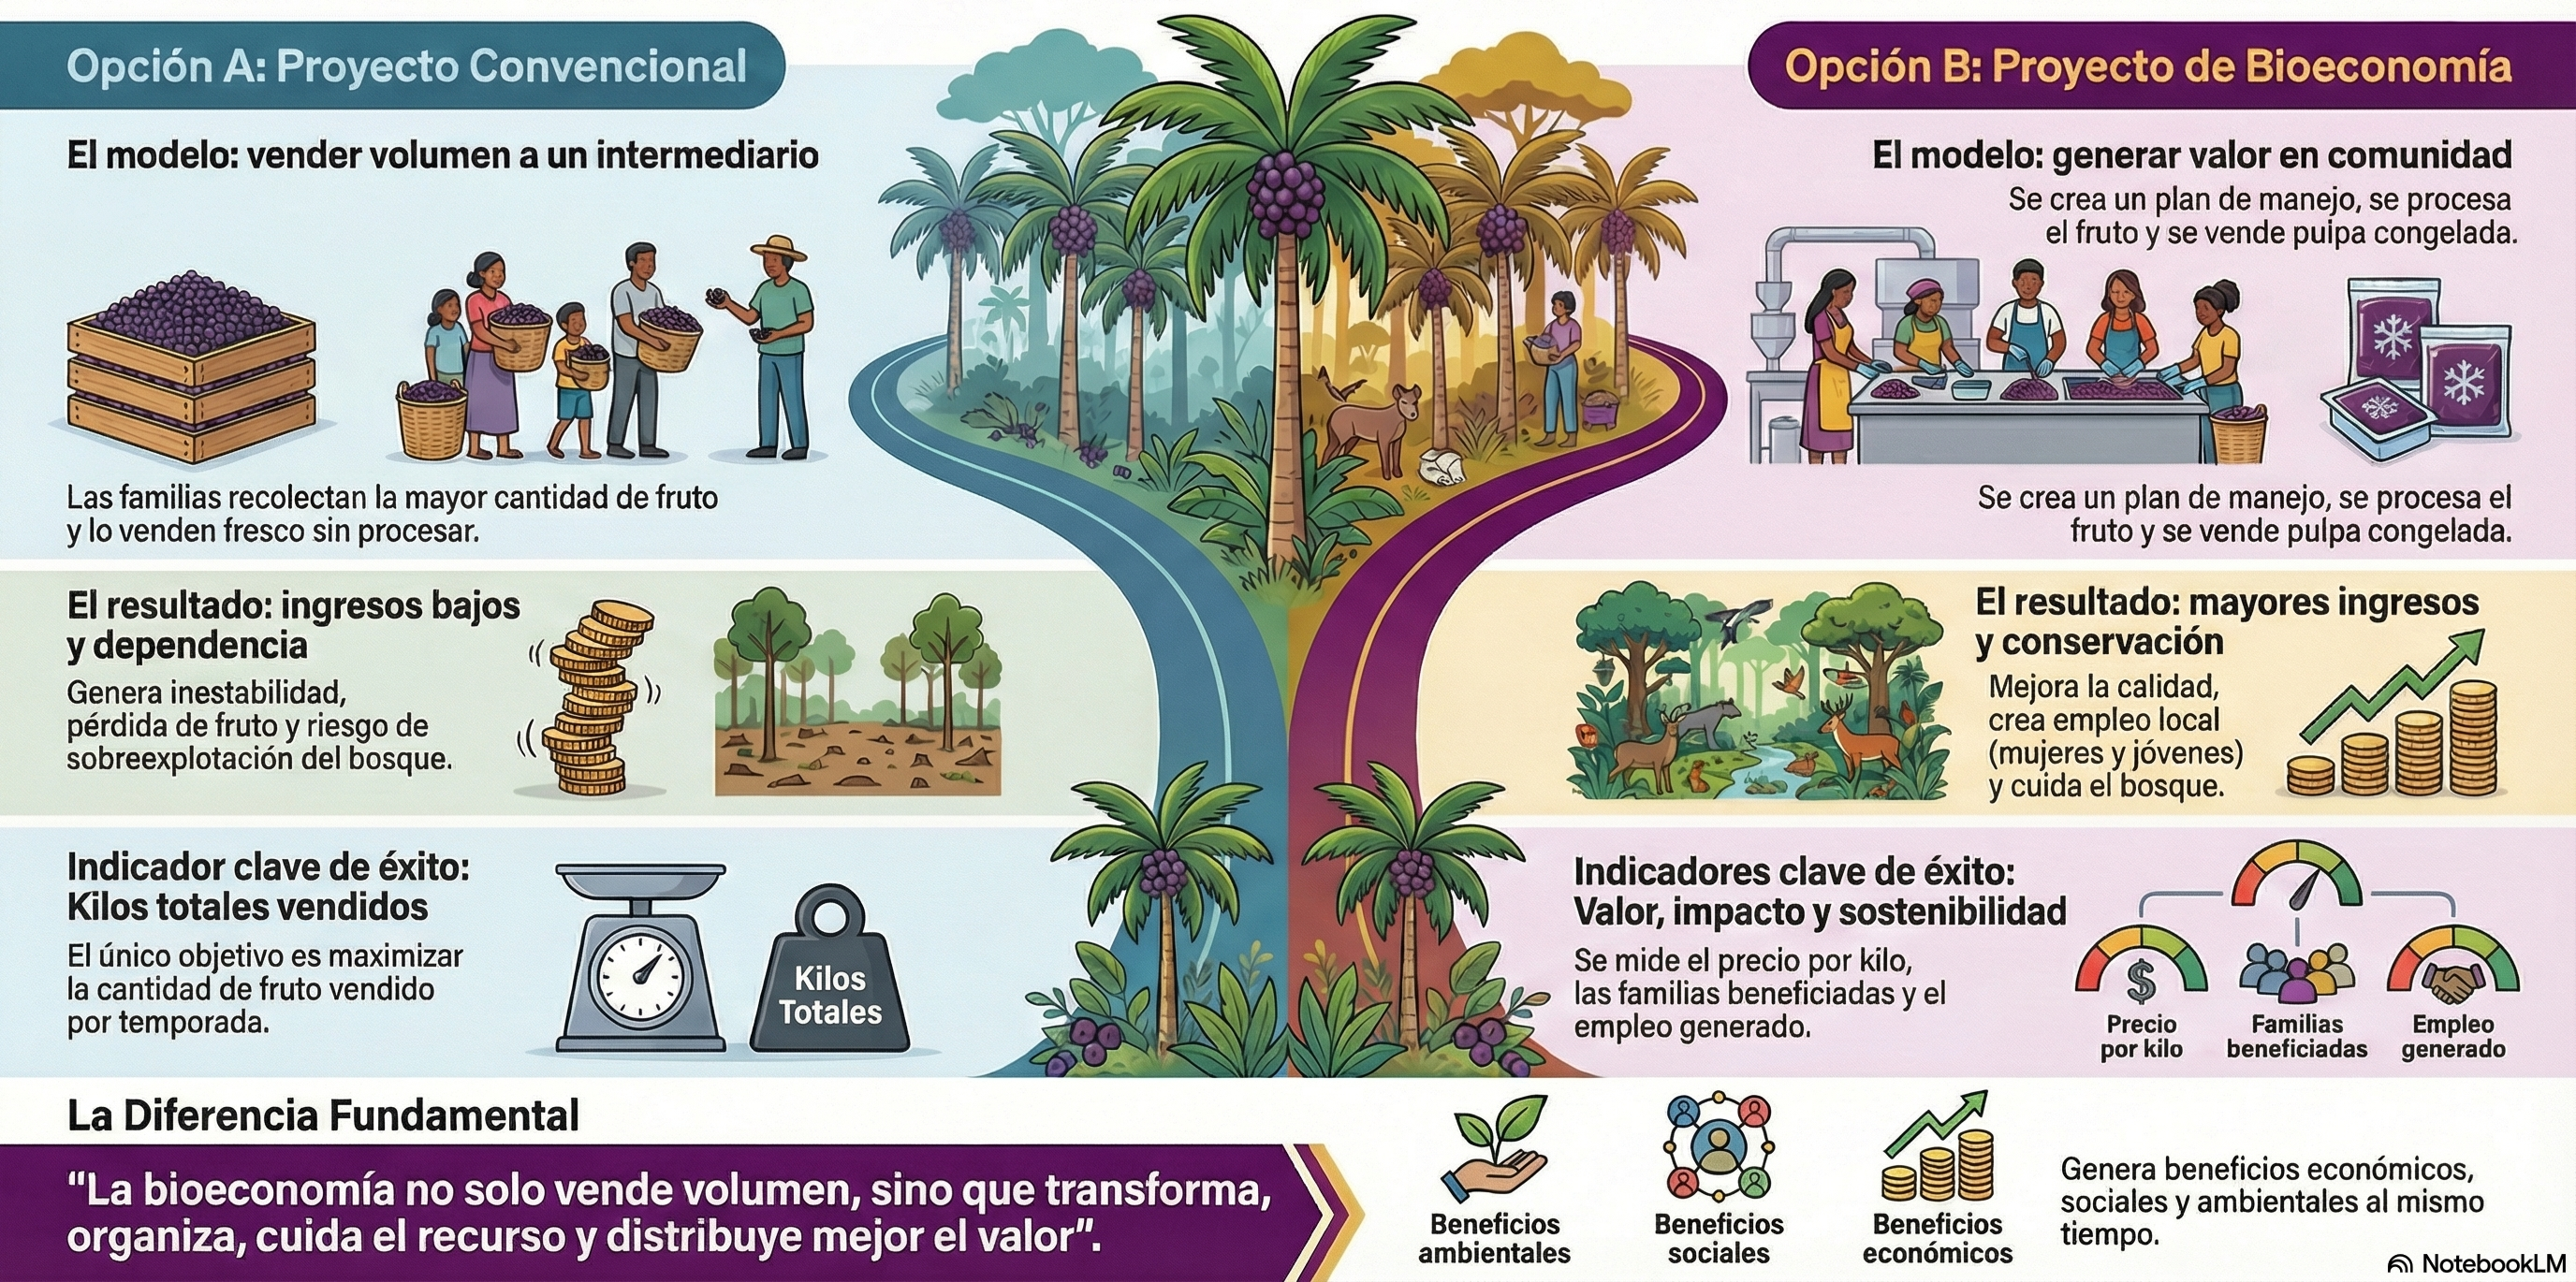
\includegraphics[keepaspectratio]{images/convencional_bioec.png}}

\end{tcolorbox}

\begin{quote}
\textbf{Lección clave:} La bioeconomía convierte la mega biodiversidad
colombiana en oportunidades de ingresos sostenibles, transformando
recursos locales renovables en productos de alto valor con triple
impacto: económico, ambiental y social.
\end{quote}

\begin{tcolorbox}[enhanced jigsaw, left=2mm, toprule=.15mm, opacityback=0, colback=white, arc=.35mm, rightrule=.15mm, leftrule=.75mm, breakable, bottomrule=.15mm, colframe=quarto-callout-tip-color-frame]
\begin{minipage}[t]{5.5mm}
\textcolor{quarto-callout-tip-color}{\faLightbulb}
\end{minipage}%
\begin{minipage}[t]{\textwidth - 5.5mm}

\vspace{-3mm}\textbf{Autoevaluación rápida}\vspace{3mm}

Marca con ✅ si aplica a tu idea

Usa un recurso biológico renovable (biomasa, biodiversidad o residuo
orgánico)

Tiene plan para no sobreexplotarlo (Plan de aprovechamiento de la
especie)

Genera empleo local inclusivo

Transforma localmente (no solo extrae y vende)

Los clientes valoran sostenibilidad y origen

Con 2--3 ✅ ya hay base sólida para explorar oportunidad; con 1 ✅
puedes pensar en un piloto pequeño; con 0 ✓ tal vez la idea necesita
ajustarse para ser realmente bioeconómica.

\end{minipage}%
\end{tcolorbox}




\end{document}
